\documentclass[a4paper]{article}

%%%%%%%%%%%%%%%%%%%%%%%%%%%%%%%%%%
% Package for making LaTeX properly handle utf8 characters set and danish language rules
\usepackage[utf8]{inputenc}
\usepackage[danish]{babel}

%%%%%%%%%%%%%%%%%%%%%%%%%%%%%%%%%%
% Package for changing to a nicer font 
\usepackage [T1]{fontenc}

%%%%%%%%%%%%%%%%%%%%%%%%%%%%%%%%%%
% Package for conctroling the text area
\usepackage[margin=2.5cm]{geometry}

%%%%%%%%%%%%%%%%%%%%%%%%%%%%%%%%%%
% Package for inserting clickable hyperlinks in pdf versions as produced by pdflatex
\usepackage{hyperref}

%%%%%%%%%%%%%%%%%%%%%%%%%%%%%%%%%%
% Package for including figures. TeX and thus LaTeX was developped before the existence of directory file-structures, but the graphicspath let's you add directories, that the \includegraphics will search.
\usepackage{graphicx}
\graphicspath{{figures/}{anotherFigureDirectory/}}

%%%%%%%%%%%%%%%%%%%%%%%%%%%%%%%%%%
% Package for typesetting programs. Listings does not support fsharp, but a little modification goes a long way
\usepackage{listings}
\usepackage{color}

\definecolor{bluekeywords}{rgb}{0.13,0.13,1}
\definecolor{greencomments}{rgb}{0,0.5,0}
\definecolor{turqusnumbers}{rgb}{0.17,0.57,0.69}
\definecolor{redstrings}{rgb}{0.5,0,0}

\lstdefinelanguage{FSharp}
                {morekeywords={let, new, match, with, rec, open, module, namespace, type, of, member, and, for, in, do, begin, end, fun, function, try, mutable, if, then, else},
    keywordstyle=\color{bluekeywords},
    sensitive=false,
    morecomment=[l][\color{greencomments}]{///},
    morecomment=[l][\color{greencomments}]{//},
    morecomment=[s][\color{greencomments}]{{(*}{*)}},
    morestring=[b]",
    stringstyle=\color{redstrings}
    }
%%%%%%%%%%%%%%%%%%%%%%%%%%%%%%%%%%
% Package for extended math settings, e.g. \eqref
\usepackage{amsmath}

%%%%%%%%%%%%%%%%%%%%%%%%%%%%%%%%%%
% These will be the title and author, as included when \maketitle is called.
\title{Opgaveskabelon}
\author{Jon Sporring }

\begin{document}
\maketitle % Insert title etc.

\section{Dette er en skabelon for en opgavebesvarelse}
Denne skabelon tænkes som et udgangspunkt til typiske opgavebesvarelser. En sådan besvarelse vil oftest bestå af et antal afsnit og underafsnit, der afspejler opgaveteksten. Husk at din lærer og instruktor ikke kan læse dine tanker, og gå derfor ud fra, at du skal være temmelig eksplicit mht.\ beskrivelse af dine overvejelser og løsning.

\section*{Opgave $m.n$}
En (del-)opgavebesvarelse indeholder som oftest:
\begin{enumerate}
\item en kort gengivelse af problemformuleringen
\item et oprids af løsningsmuligheder
\item en kort beskrivelse af de overvejelser og argumenter, som har ledt til løsningen
\item den endelige løsning
\end{enumerate}
Argumentation og løsning vil oftest blive styrket af en eller flere figurer som f.eks.\ Figur~\ref{fig:eksempel}.
\begin{figure}
  \centering
  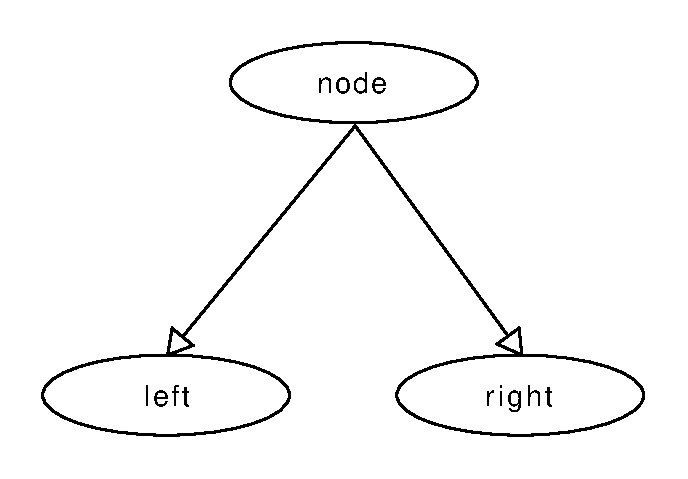
\includegraphics[width=0.6\linewidth]{treeNode} % We don't need to specify the filename suffix
  \caption{En trætype: knude har 2 børn, som enten er tom eller en knude.}
  \label{fig:eksempel}
\end{figure}
Oftest indeholder datalogiske opgavebesvarelser også kode stumper som f.eks.\ Figur~\ref{fig:fsharpCodeExample}
\begin{figure}
  \lstset{language=FSharp}
\begin{lstlisting}
(* Fibonacci Number formula *)
let rec fib n =
    match n with
    | 0 | 1 -> n
    | _ -> fib (n - 1) + fib (n - 2)
\end{lstlisting}
  \caption{An example of a program listing. Sometimes this is included in a float, other times inline in the text.}
  \label{fig:fsharpCodeExample}
\end{figure}
Det kan også hænde at en besvarelse indeholder ligninger, som f.eks.\ vist i \eqref{eq:anEquation}.
\begin{equation}
  \label{eq:anEquation}
  f(x)=ax^2+bx+c
\end{equation}
\end{document}

